\textcolor{blue}{
    As we have motivated \textit{query split} and introduced all the details, we evaluate its performance on real-world workload in this section. We first describe how our experiments are organized (Section \ref{S51}). Next, we evaluate the performance impact of different query splitting algorithms and execution order decisions (Section \ref{S52}). Then, we investigate the sensitivity of heuristic-based order algorithms for the accuracy of cardinality estimation (Section \ref{S53}). And we compare a fine-tuned \textit{query split} implementation with baselines (Section \ref{S54}). We also discuss the materialization overhead among re-optimization techniques (Section \ref{S55}). Last, we discuss the influence of collecting different run-time statistics (Section \ref{S56}).
}
\subsection{Experiment Setup} \label{S51}
\textcolor{blue}{
    Our experiments are performed on a 64-bit Windows 10 computer with an Intel Core i9-10900K CPU (3.70 GHz) and 128GB RAM. We use the source code of PostgreSQL 12.3 as the basis for our implementations. In PostgreSQL, ”analyze” is the command that manually orders the optimizer to collect statistics for base relations. We call the same routine to gather the run-time statistics. In addition, we set max parallel workers to 0, so the CPU only uses one core during query processing. Furthermore, we increase the effective cache size to 8GB, and other parameters are set as default.
}\par
    We use Join Order Benchmark (JOB) \cite{JOB} as our experiment workload. JOB is a real-world workload over the IMDB dataset and has a high value for evaluating the performance of RDBMS. JOB has 113 queries, and 91 of them have non-empty results. We run these 91 queries and record their latency as reported by PostgreSQL.\par
    We have released the source code of \textit{query split} that we used in experiments on Github. \footnote[2]{https://github.com/zhaojy20/break-up-pipeline.}

\subsection{Different Implementations of sub-query perspective} \label{S52}
\textcolor{blue}{   
    We first evaluate the performance of different implementations of \textit{query split}. We test the total end-to-end latency for different sub-query splitting algorithms with all execution order decision strategies, and the result is shown in Table \ref{T3}. There are B+ tree indexes on both primary and foreign key attributes.
}
    \begin{table*}[htb]
        \caption{Total latencies for different implementations on JOB}
        \label{T3}
        \begin{tabular}{c|ccc}
            \toprule
            \diagbox{Function}{Latency(s)}{Strategy} & \textit{RelationshipCenter} & \textit{MinSubquery} &  \textit{EntityCenter} \\
            \midrule
            $cost(q)$                                &              421            &          463         &            378         \\
            $row(q)$                                 &              348            &          474         &            407         \\         
            $row\_hybrid(q)$                         &              295            &          427         &            350         \\
            $hybrid\_sqrt(q)$                        &              328            &          418         &            339         \\
            $hybrid\_log(q)$                         &              327            &          428         &            349         \\
            $global\_sel$                            &              356            &          401         &            413         \\
            \bottomrule
        \end{tabular}
    \end{table*}\par
    From Table \ref{T3}, we can conclude that both query splitting algorithms and execution order decisions influence the end-to-end latency. \textit{Minsubquery} uses the longest time for every execution order among query splitting algorithms. This result may be due to too much materialization, which apparently slows down the execution speed. The result suggests that \textit{Minsubquery} is not a good choice for query splitting. In most cases, \textit{RelationshipCenter} has the lowest latency, which proves our proposal that constraining the sub-query size can benefit the query execution latency.\par
\textcolor{blue}{
    Next, we observe that the end-to-end latency between five execution order decisions also changes significantly. $row(q)$, $cost(q)$, and $hybrid\_log(q)$ are the worst sub-query order selection strategies, as there is a gap between the weights given on row and cost. On the other hand, $hybrid\_sqrt(q)$ and $row\_hybrid(q)$ perform pretty closely. This finding indicates that the concrete parameters are unimportant as long as we consider current and future benefits with similar weights.
}\par
\textcolor{blue}{
    Meanwhile, although $global\_sel$ provides a global view, it does not outperform the heuristic rule based methods. Actually, the performance of $global\_sel$ is worse than heuristic rule based methods for most query splitting algorithms. This result proves our statement that the global plan may mislead the re-optimization. As a result, the execution order based on the global plan performs poorly.
}\par

\subsection{Sensitivity of Order Algorithm for CE Accuracy} \label{S53}
\textcolor{blue}{
    As our ranking functions take cardinality as an input, they may be sensitive to the accuracy of cardinality estimation. Therefore, we do the following experiments to investigate how the cardinality estimation error influences heuristic-based execution order decision algorithms.
}\par
\textcolor{blue}{
    The first step of this experiment is to get the accurate cardinality of every intermediate join result and the execution plan based on it. To this end, we make an optimal optimizer by following methods. We first execute all the possible sub-expression of the given query in advance and record their accurate cardinality. And then, we inject these actual values into the PostgreSQL optimizer by the method proposed by Cai, Balazinska, and Suciu \cite{PessimisticCE}. Thus, the optimizer knows the actual size of each intermediate relation and can make the optimal plan.
}\par
\textcolor{blue}{
    Then, we add noise to the accurate cardinality in order to get the cardinality with the artificial error. The formula for adding error is shown below, where $G(m, n)$ is a Gaussian distribution with mean $m$ and standard error $n$.
}
    $$ est\_card = 2^{G(m, n)} * true\_card $$\par
\textcolor{blue}{
    The total end-to-end latency of different execution order decision algorithms with different errors is shown in Figure \ref{F9}. From Figure \ref{F9}, we can see that although the latency performance degrades along with the increasing of cardinality estimation error, the relationship between ranking functions is invariant: the end-to-end latency of $cost(q)$, $row(q)$, and $hybrid\_log(q)$ is more than the other two ranking functions, i.e., $hybrid\_sqrt(q)$ and $row\_hybrid(q)$. This result indicates that we should consider both the row and cost of the sub-plan and give them similar weights. Moreover, the performance of $hybrid\_sqrt(q)$ and $row\_hybrid(q)$ keeps quite close throughout, the same as the conclusion from Table \ref{T3}.
}
    \begin{figure*}[htb]
        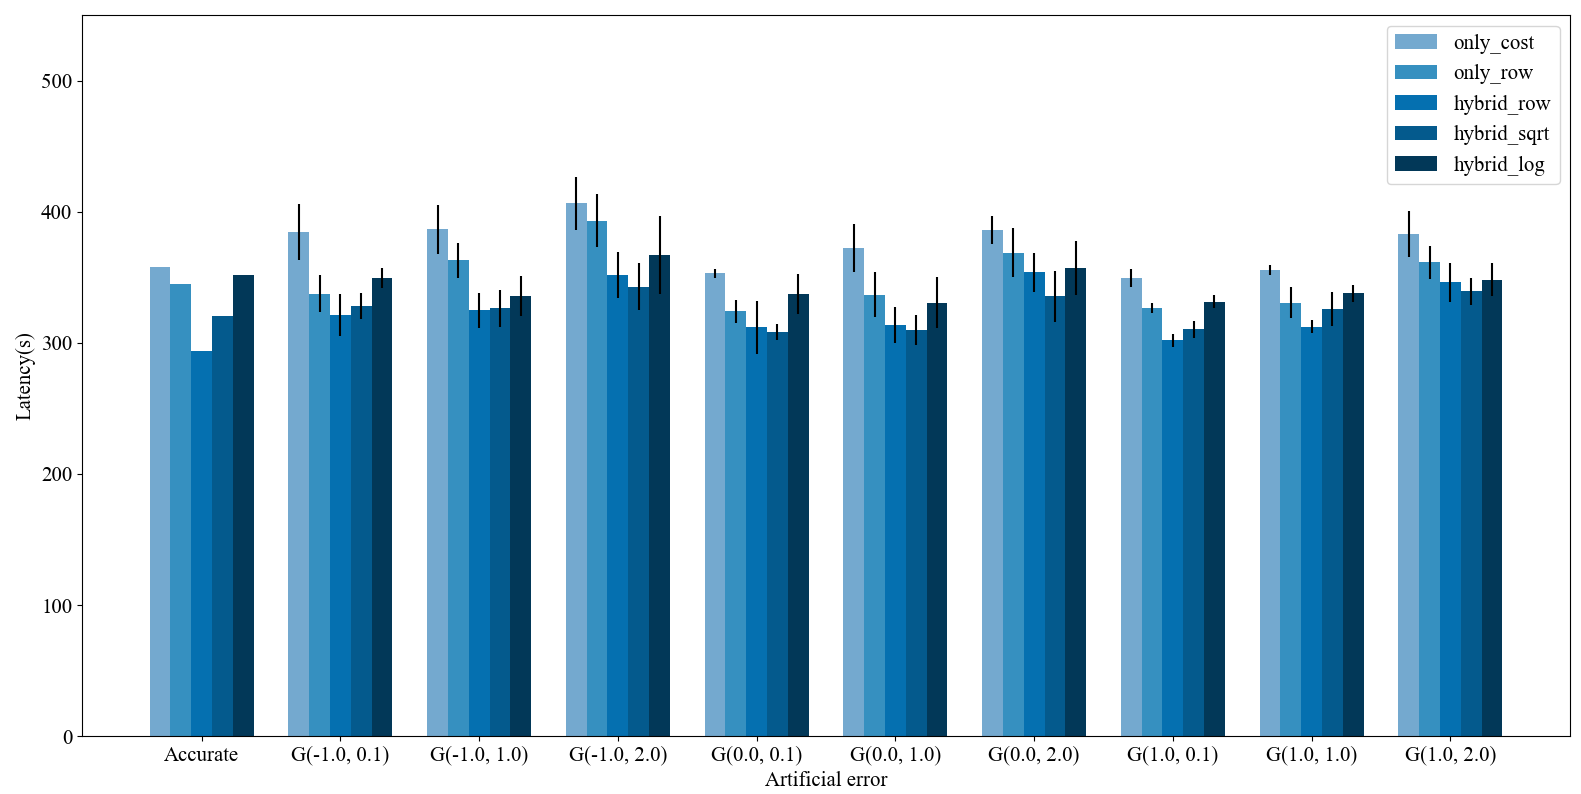
\includegraphics[width=\linewidth]{./pic/Figure9.png}
        \centering
        \caption{Latency of different heuristic-based algorithms under true cardinality and different cardinality estimation error}
        \label{F9}
        \Description{}
    \end{figure*}\par

\subsection{Performance of Query Split} \label{S54}
\textcolor{blue}{
    We further compare \textit{query split} with several baselines. They are 
    \begin{itemize}[leftmargin = 15pt]
        \item Original PostgreSQL.
        \item Optimal optimizer: we have described optimal optimizer above.
        \item Reopt. \cite{Reopt}: A re-optimization technique that only materializes blocked operators and then re-optimizes.
        \item Pop \cite{Pop}: A re-optimization technique materializes both blocked operators and outer sides of nest-loop join.
        \item Query incremental execution (QIE) \cite{QIE}: A re-optimization technique materializes the operator that has the highest cardinality estimation error.
        \item Perron19': A re-optimization technique, which is a brief implementation of the simulation conducted by Perron et al \cite{MichaelStonebraker}. Materializes the nodes that join two relations at a time and then re-optimizes.
        \item USE \cite{USE}: A cardinality estimation technique. Executing the non-expanding operators (i.e., filters and Pk-Fk joins) first and selecting join order by the upper bound of the join instead of cardinality.
        \item Pessimistic CE \cite{PessimisticCE}: A cardinality estimation technique. A worst-optimal cardinality estimator leverages randomized hashing and data sketching to estimate the upper bounds of join size. And using that upper bound to replace the role of cardinality in query optimization. 
    \end{itemize}
}\par
    According to above conclusion, we choose \textit{RelationshipCenter} with $hybrid\_row(q)$ to represent \textit{query split} in the rest of paper, which has the least total end-to-end latency among all implementations.\par
\textcolor{blue}{
    As some source codes of these baselines are not implemented in PostgreSQL, we implement them in PostgreSQL by ourselves according to their algorithms. The parameter configuration is the same as the experiment setup in their paper.
}\par
\textcolor{blue}{
    Figure \ref{F10} and \ref{F11} show the total latency of \textit{query split} and above baselines in two kinds of JOB. One is only the indexes on primary key attributes are available (JOB with Pk index) and another is indexed on both primary key and foreign key (JOB with Pk + Fk index). We set a timeout of total latency as 1000 seconds.
}
    \begin{figure}[htb]
        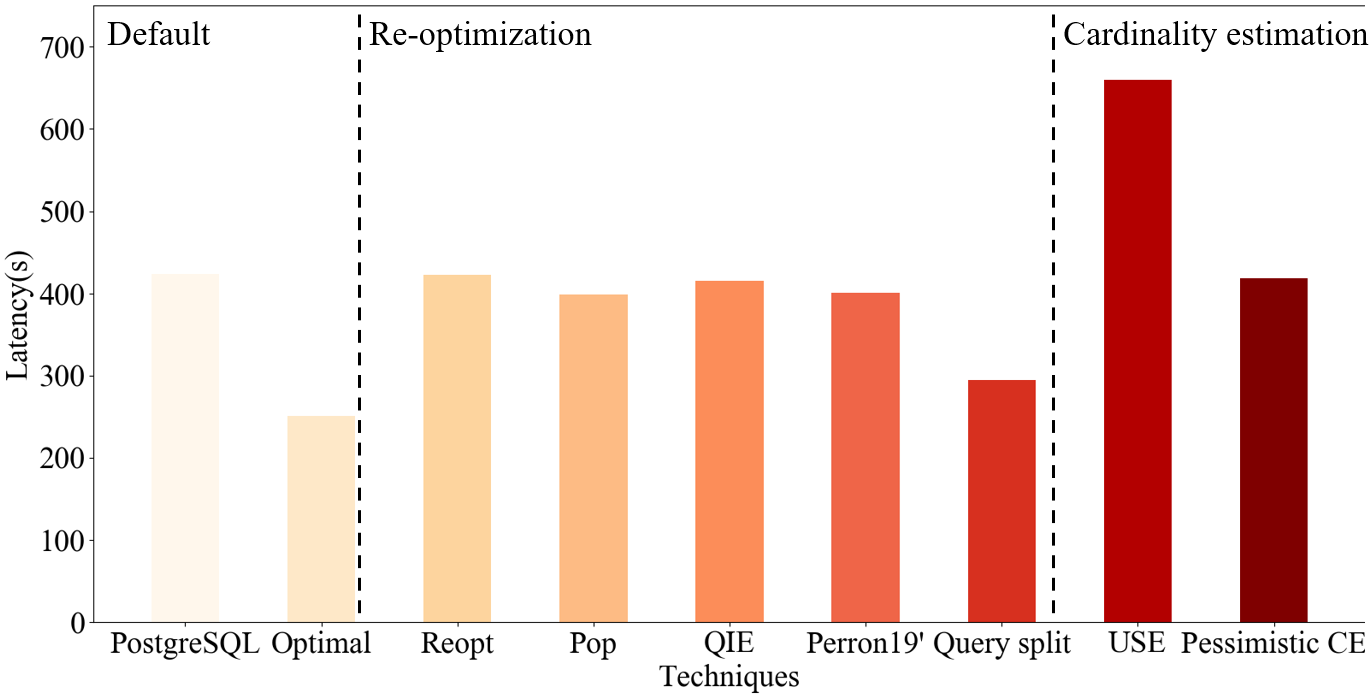
\includegraphics[width=\linewidth]{./pic/Figure10.png}
        \centering
        \caption{Total latency comparison in JOB with Pk + Fk index}
        \label{F10}
        \Description{}
    \end{figure}
    \begin{figure}[htb]
        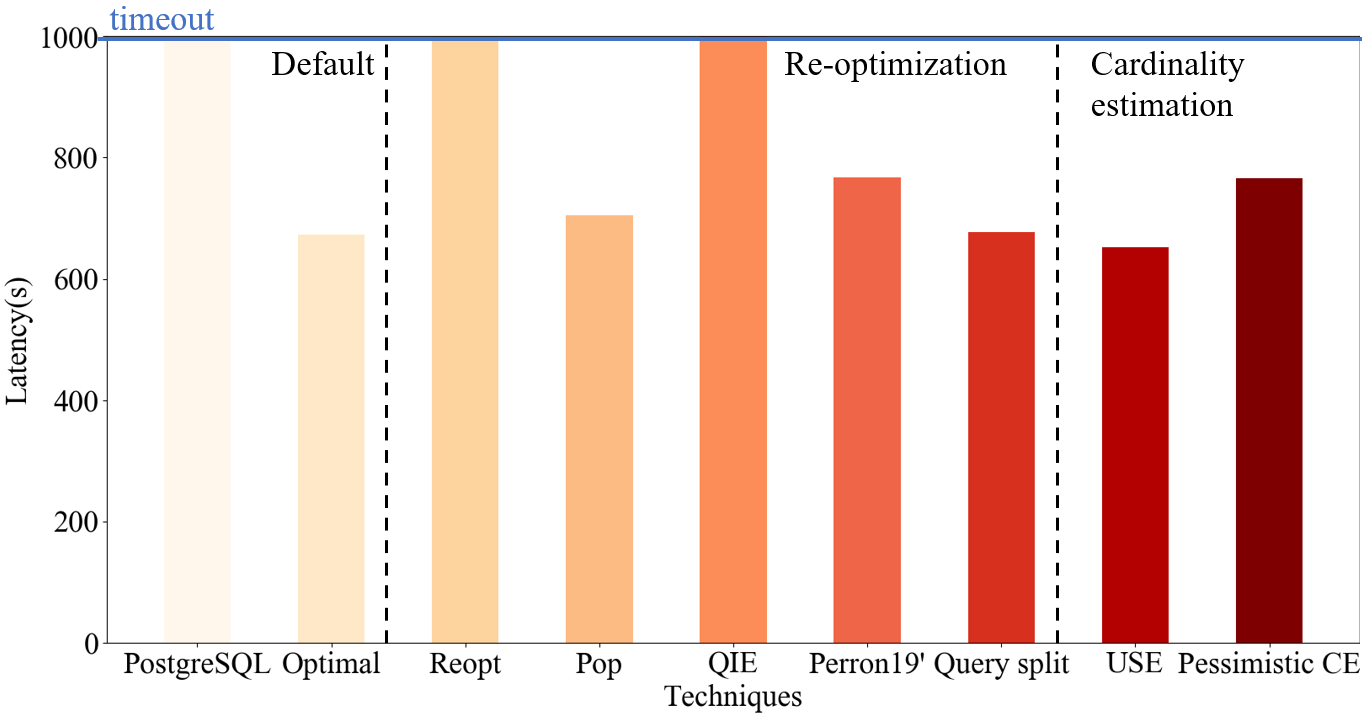
\includegraphics[width=\linewidth]{./pic/Figure11.png}
        \centering
        \caption{Total latency comparison in JOB with Pk index}
        \label{F11}
        \Description{}
    \end{figure}\par
\textcolor{blue}{
    We can draw two conclusions from the above figures. First, \textit{query split} outperforms other query processing techniques. In both Pk-indexed JOB and Pk + Fk indexed JOB, \textit{query split} has a significant speedup for total latency compared to PostgreSQL, other re-optimizations, and new cardinality estimation techniques, which verifies the effectiveness of \textit{query split}. And \textit{query split} is very close to the optimal result. Although there is still a gap between \textit{query split} and \textit{optimal plan} in Pk + Fk indexed JOB, the gap is mainly caused by a few queries, whereas the latency of other queries in \textit{query split} is close to \textit{optimal plan}. And another reason is that the more indexes are available, the harder the job of the query optimizer becomes \cite{JOB}. The result suggests that by proper splitting algorithm and execution order decision, the plans we execute each iteration are more similar to sub-trees of the optimal plan.
}\par
\textcolor{blue}{
    Second, no index on foreign key attributes increases the cost of a bad plan, and therefore the effect of misleading global plans is revealed. The techniques that have the best performance in JOB with Pk index are USE and query split, which both discard the global plan totally. And other re-optimization techniques do not perform well because they are more or less influenced by the terrible part of the global plan.
}\par
    Another implication is that the accuracy of cost model would affect the system performance. We observe that in JOB (Pk index), the latency of \textit{optimal plan} is longer than USE. The reason for this counter-intuitive phenomenon is that the estimation error of cost model, which leads the optimizer to select a sub-optimal physical operator. As the number of configuration parameters that can be tuned in PostgreSQL is limited, it is impossible to tune a perfect cost model. The issue of cost model accuracy is beyond the scope of this paper, and we merely point it out as a potential direction for future research.

\subsection{Materialization Overhead} \label{S55}
\textcolor{blue}{
    All re-optimizations need to materialize the intermediate results as temporary tables. Hence, materialization overhead is an important metric of re-optimization.
}\par
\textcolor{blue}{
    We test the average memory used for materializing the intermediate results of all re-optimization techniques as materialization overhead, and the results are shown in Table \ref{T4}. And we use JOB with Pk + Fk index for the experiment.
}
    \begin{table*}[htb]
        \caption{Materialization overhead of re-optimization techniques}
        \label{T4}
        \begin{tabular}{c|c|c|c}
            \toprule
            Re-optimizations       &  Average overhead & Average re-optimize times & Memory consumption per materialization \\
            \midrule
            \textit{Query split}   &     15.401 MB     &            2.66           &  5.79 MB \\
            Perron19'              &     72.445 MB     &            6.59           & 10.99 MB \\
            Reopt                  &      9.096 MB     &            0.21           & 43.31 MB \\
            Pop                    &     32.396 MB     &            4.62           &  7.01 MB \\
            QIE                    &     45.380 MB     &            3.11           & 14.59 MB \\
            \bottomrule
        \end{tabular}
    \end{table*}\par
\textcolor{blue}{
    From Table \ref{T4}, we can see that \textit{query split} and reopt have low average materialization overhead. However, the overhead of reopt is low because re-optimization is triggered rarely in these two re-optimization techniques. Hence, by calculating the memory consumption per materialization, we find that \textit{query split} has the most efficient memory usage. This is because \textit{query split} controls the result size of sub-query by a specially-designed splitting algorithm, while other re-optimization techniques fail to control the intermediate result sizes.
}

\subsection{Collecting different Run-time Statistics} \label{S56}
\textcolor{blue}{
    The run-time statistics we discuss in the paper include the true cardinality and fine-grained statistics like the most common values, histogram, or the number of distinct values. An interesting question is whether those fine-grained statistics are indispensable for refining execution plans, and we discuss this question in this subsection.
}\par
\textcolor{blue}{
    We test all the re-optimization techniques with and without collecting fine-grained statistics after each materialization. Without collecting fine-grained statistics, the optimizer only knows the size of the intermediate result. As we described before, fined-grained statistics are collected by calling the functions used by PostgreSQL ``analyze" command. The latency of JOB with or without fine-grained statistics is shown in Figure \ref{F12}, and we use JOB with Pk + Fk index for the experiment.
}
    \begin{figure}[htb]
        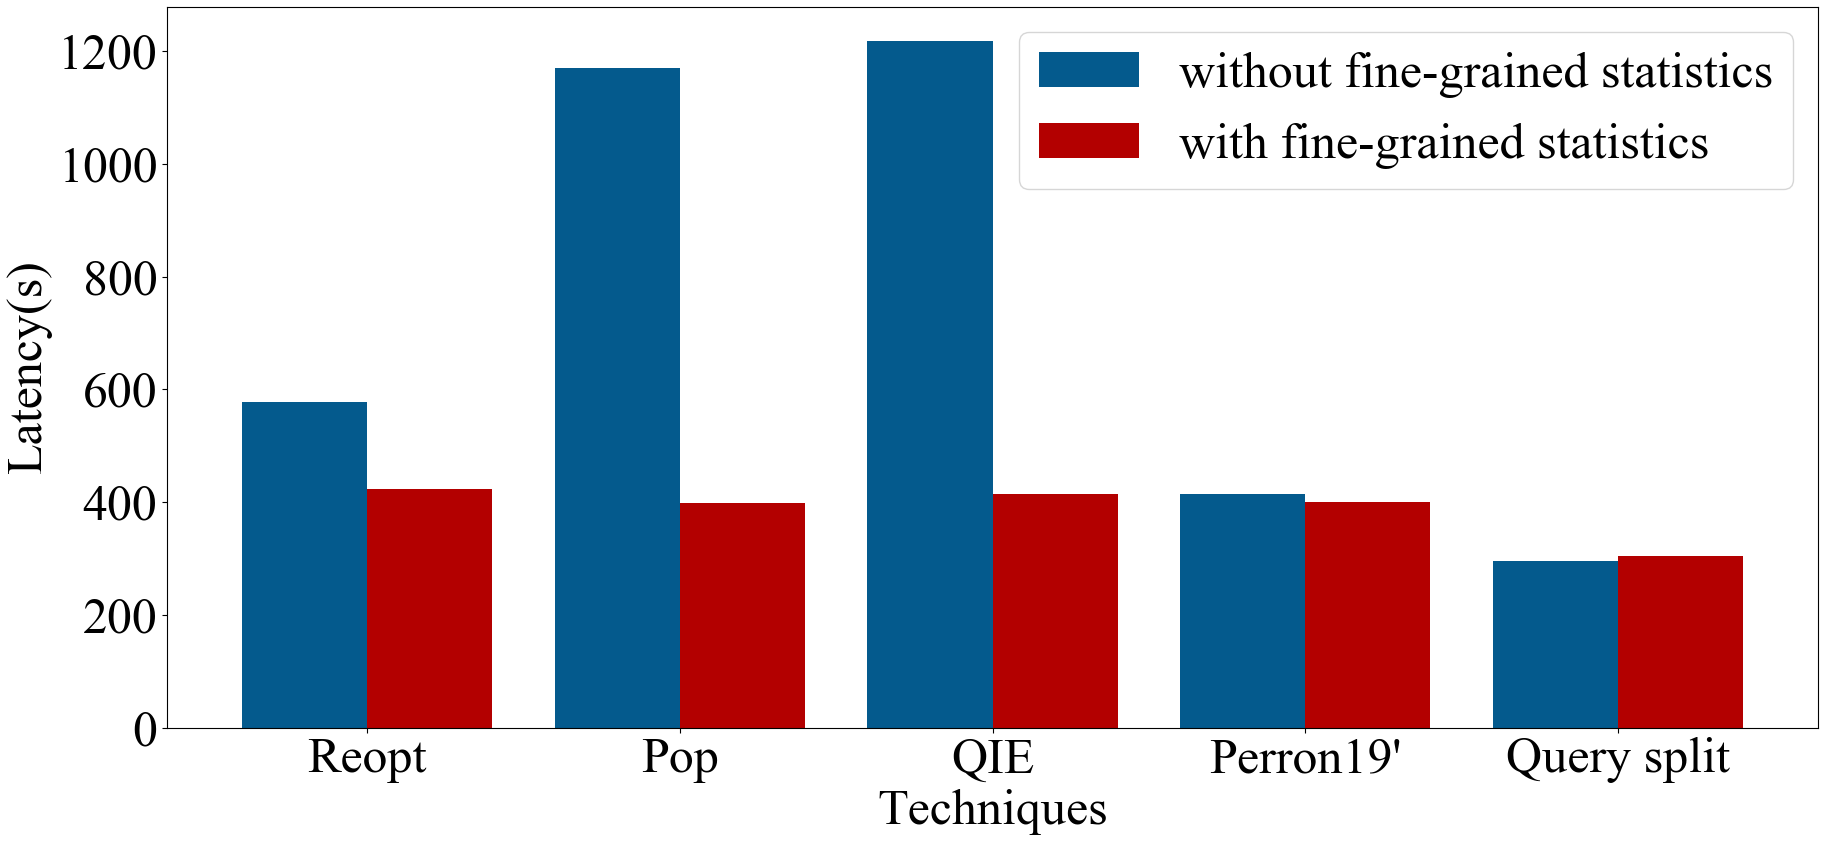
\includegraphics[width=\linewidth]{./pic/Figure12.png}
        \centering
        \caption{Total latency with and without fine-grained statistics}
        \label{F12}
        \Description{}
    \end{figure}\par
\textcolor{blue}{
    From Figure \ref{F12}, we can see that \textit{query split} and Perron19' perform well even without fine-grained statistics during run-time. However, most re-optimization techniques depend heavily on fine-grained statistics to help refine the remaining query.
}